\documentclass{report}
\usepackage{graphicx}
\usepackage{placeins}
\title{Lab 1: Battery Evaluation}
\date{September 9th, 2022}
\author{Brady Moore \\
    Nataly Panczyk}

\begin{document}
\maketitle
\section{Statement of Purpose}
In ECE 205 lecture, we deal with ideal voltage and current sources, but in real life, there are no such things.
In this lab, we will use a battery, which is a device which converts chemical energy into electrical energy.
Even though we typically think of batteries as ideal voltage sources, we will characterize ways in which the battery differs from the ideal voltage source.

\section{Procedure}
\begin{figure}[htpb]
    \centering
    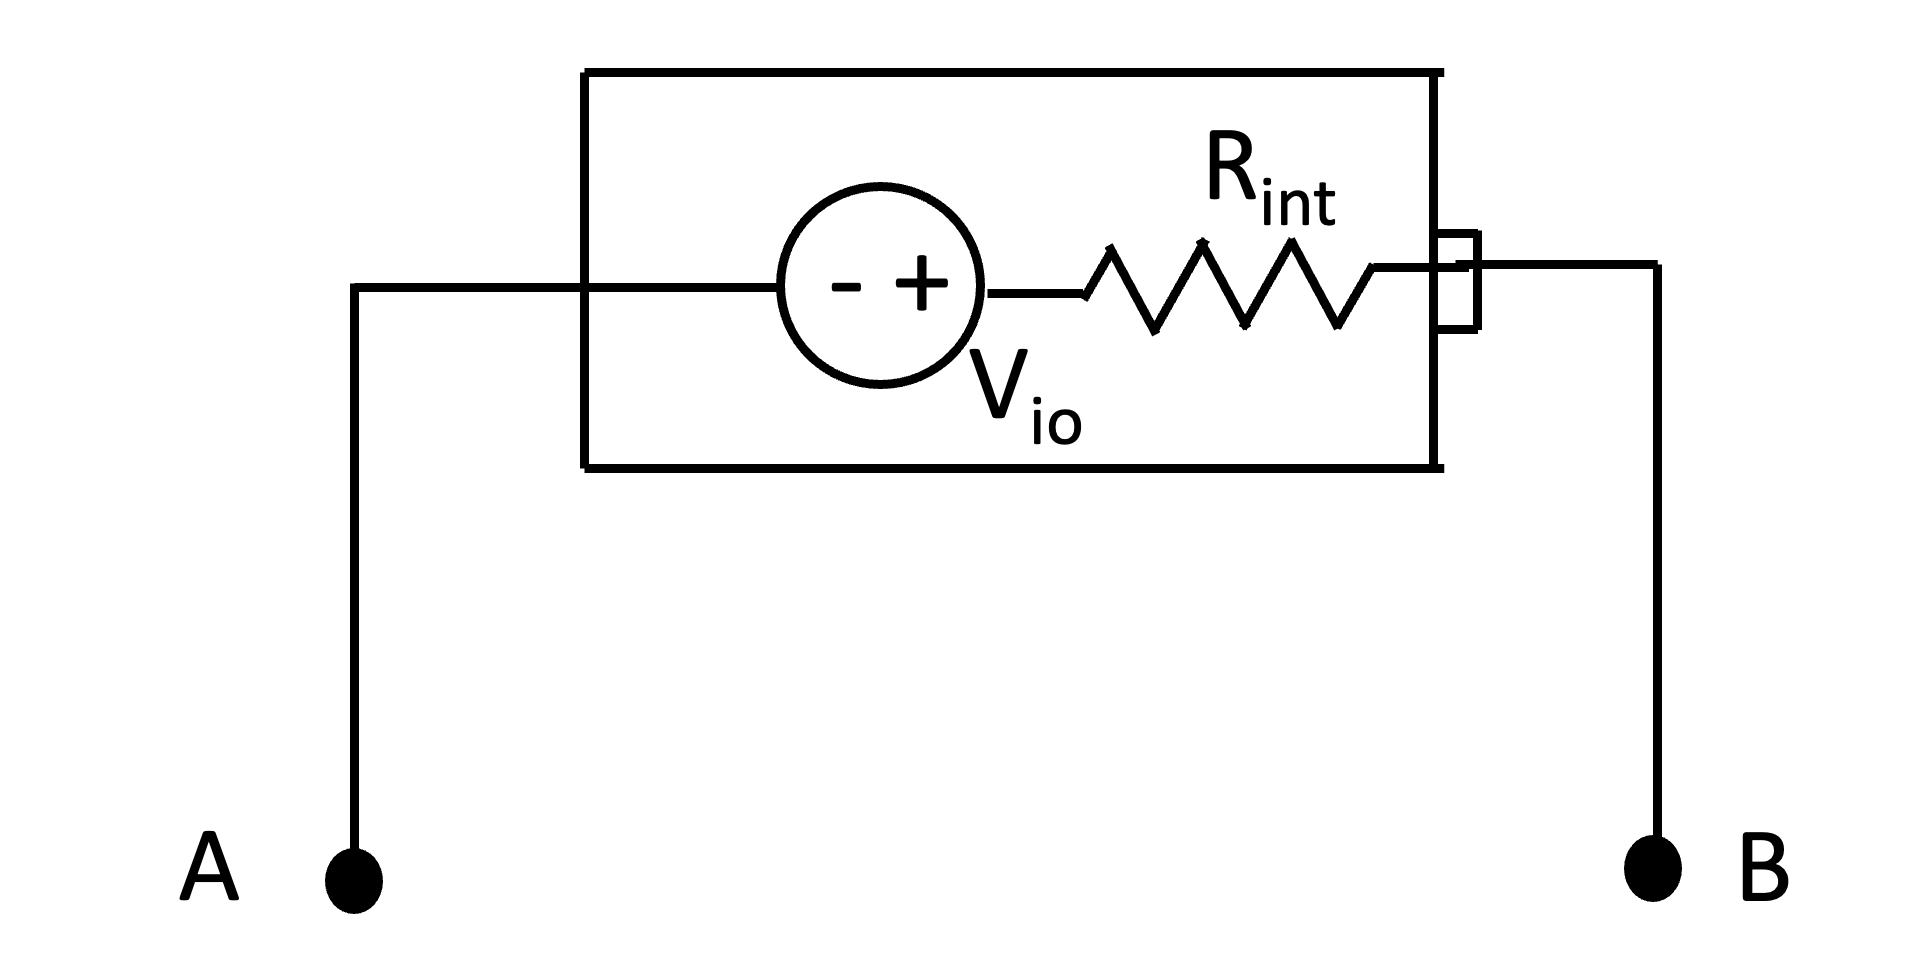
\includegraphics[width=0.8\textwidth]{SchematicA.png}
    \caption{A schematic showing how $V_{oc}$ was measured.}
    \label{fig:SchemA}
\end{figure}
\begin{figure}[htpb]
    \centering
    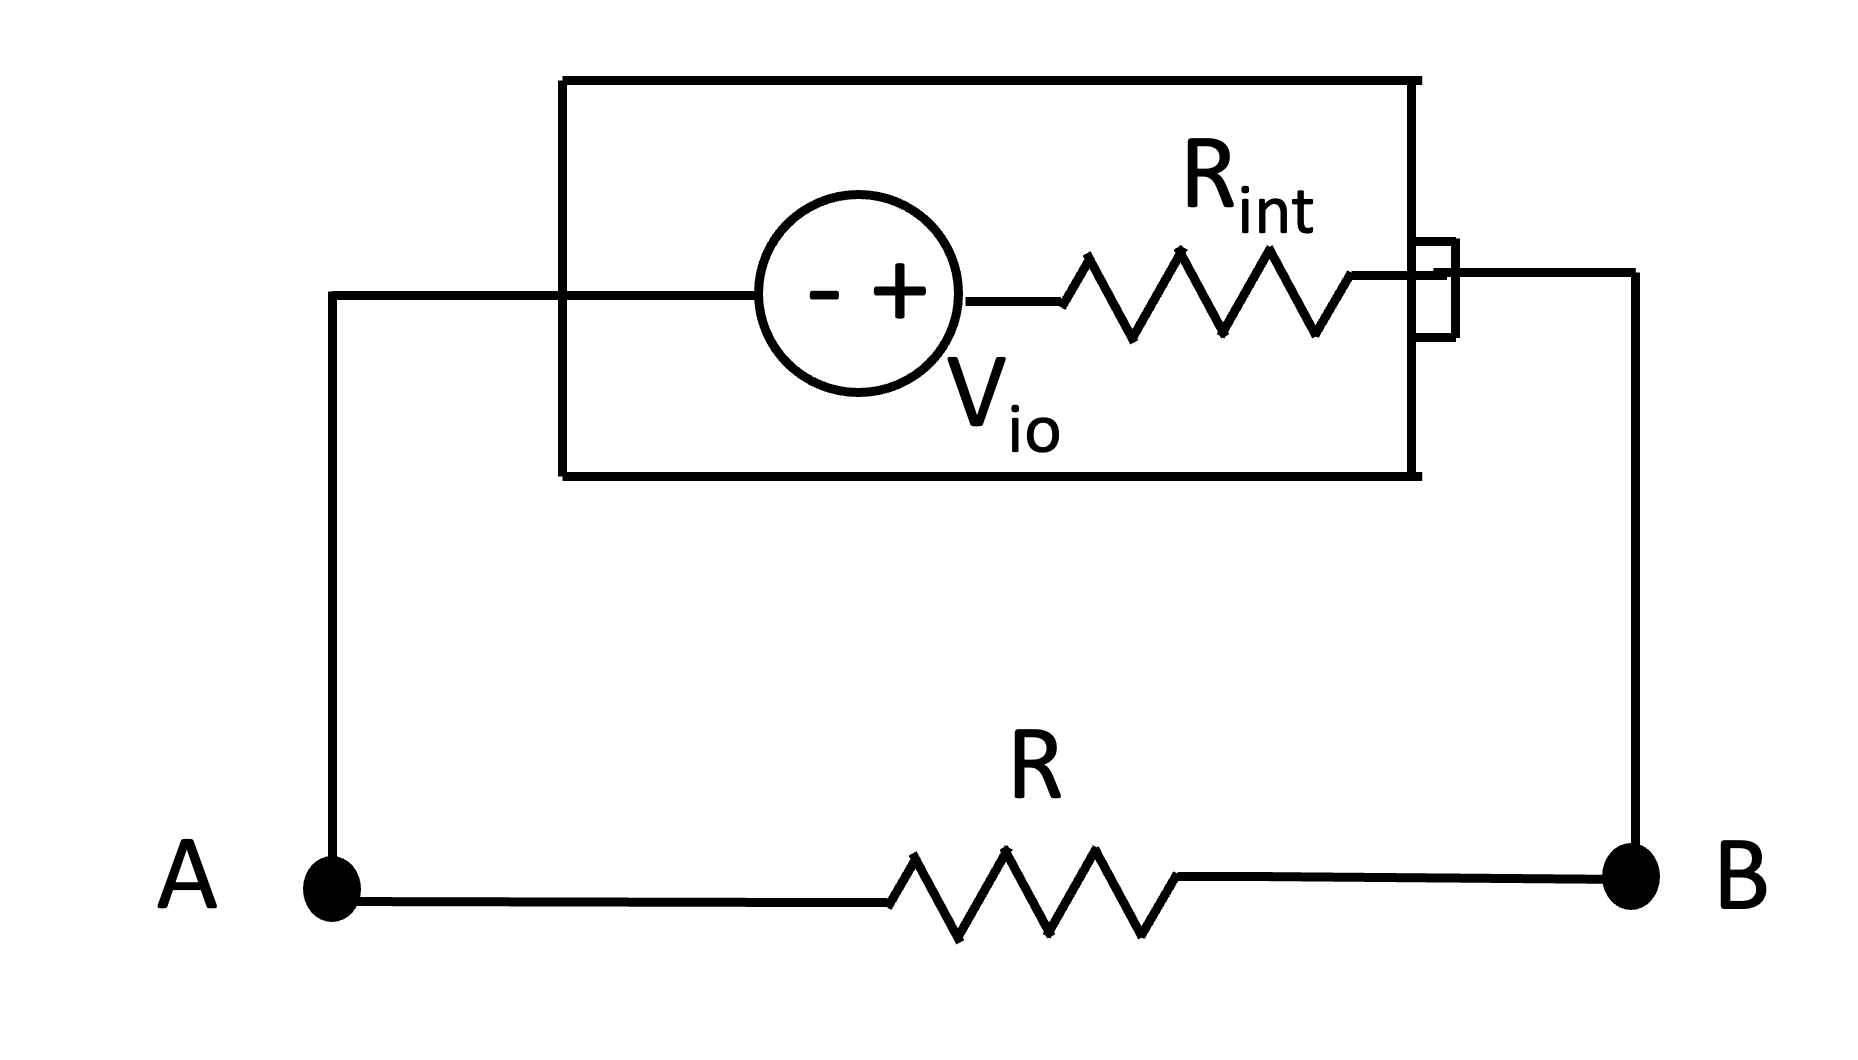
\includegraphics[width=0.8\textwidth]{SchematicB.png}
    \caption{A schematic showing how $V_{ab}$ was measured.}
    \label{fig:SchemB}
\end{figure}
\section{Raw Data}
\begin{table}
    \begin{center}
    \caption{Experimental values of $V_{oc}$ and $V_{ab}$ for all three batteries. The current and $R_{int}$ columns are calculated using Eq.~\ref{}}
    \label{tab:results}
    \begin{tabular}{|c c c c c|}
        \hline
        Battery & $V_{oc} [V]$ & $V_{ab} [V]$ & $ I[A]$ & $R_{int} [\Omega]$\\
        \hline
        A      &   1.6044    &  1.5918     &  0.015918     &  0.79155 \\
        B   & 1.6072    & 1.6025 &  0.016025 & 0.2933 \\
        C   & 1.6083    & 1.5865    & 0.015865  & 1.3741 \\
        \hline

    \end{tabular}
    \end{center}
    \end{table}
\section{Analysis}
The voltage meausered across the battery is the open load voltage, $V_{oc}$,because there is no load or current flowing.
$V_{ab}$ is the voltage drop across the 100 $\Omega$ resistor.
$V_{ab}$ can be used to find the current flowing through the circuit according to Ohm's Law Eq.~\ref{ohms_law}.
The current in addition to $V_{oc}$ can be used to calculate the internal resistance according to the following equation:
\begin{equation}
    V_{oc} = I(R+R_{int})
\end{equation}
where $R$ is the resistance of the added resistor.
For this lab $R = 100 \Omega$.
\begin{equation}
    R_{int} = \frac{V_{oc}}{I}-R
\end{equation}
The calculated $R_{int}$ values are tabulated in Table~\ref{tab:results}.
\section{Conclusion}
\end{document}
